% NeuroCam manual - Overview
% Written by Christopher Thomas.
% Copyright (c) 2021 by Vanderbilt University. This work is released under
% the Creative Commons Attribution-ShareAlike 4.0 International License.

\chapter{Overview}
\label{intro}

The NeuroCam system is a computer-controlled camera network that collects
footage of a subject interacting with a game (or other apparatus).
It was commissioned by the Attention Circuits Control Laboratory
(\verb+http://accl.psy.vanderbilt.edu/+)
to facilitate their experiments.

A system diagram is shown in Figure \ref{fig-system}, below:

\begin{figure}[h]
\begin{center}
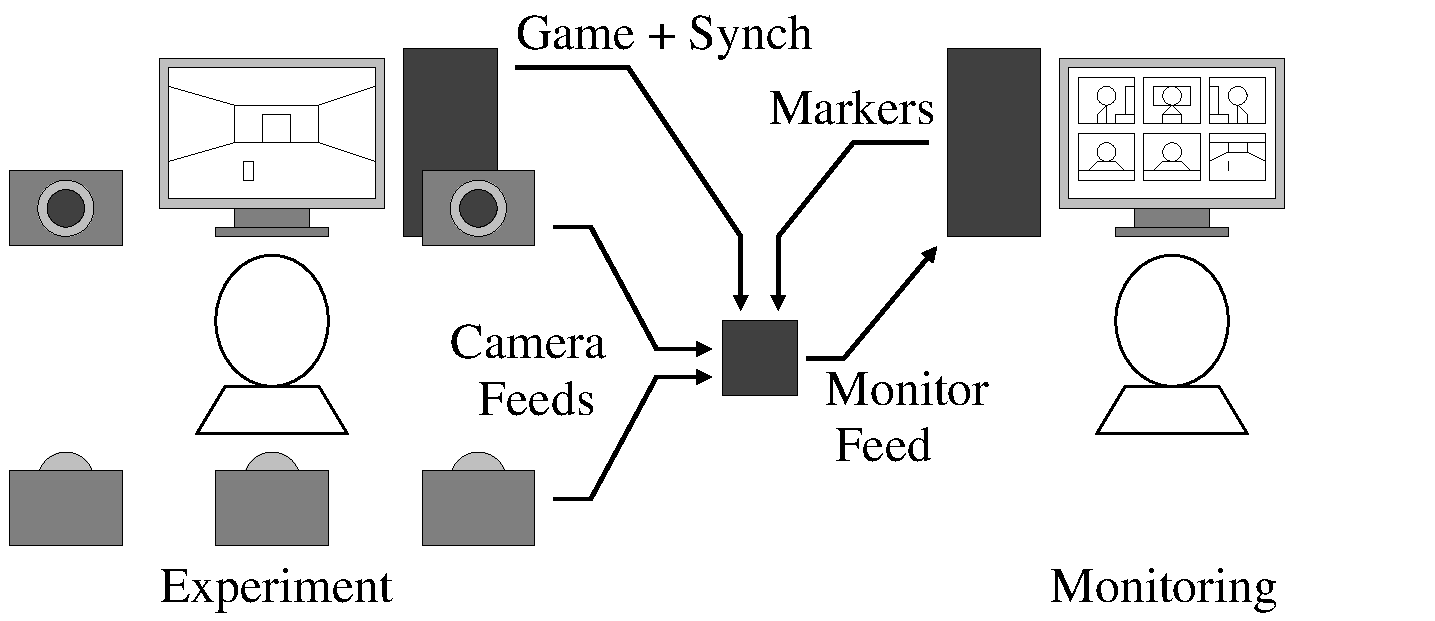
\includegraphics[width=0.95\textwidth]{figs/system-ext.pdf}
\end{center}
\caption{System block diagram.}\label{fig-system}
\end{figure}

The NeuroCam system processes several types of data and events (described
in detail in later sections):

\begin{itemize}

\item It collects frame data (with timestamps) from several cameras.

\item It collects streamed video data from the game machine.

\item It accepts web connections from authorized computers for control and
monitoring.

\item It provides a ``monitoring'' feed to the control computer showing
all video streams.

\item It records ``marker'' events when interface buttons are clicked on
the monitoring web page.

\item It records digital (TTL) signals from external equipment.

\item It accepts TTL ``start'' and ``stop'' signals from external equipment.

\item It offers collected data for examination, download, and
post-processing via a web interface after experiments have completed.

\end{itemize}

% NOTE - We can't mbox verbatim commands, so manually add line breaks.
To get started, connect an authorized machine to the ``\verb+neurocam+''
network and point it to \linebreak
``\verb+http://192.168.1.+\textit{(value)}''
(the IP address given on the sticker on the NeuroCam machine).

%
% This is the end of the file.
